\paragraph{}
Para o circuito projetado utilizando-se das equações de transferencia (acima) e ensaiado no programa \emph{Simulink} do \emph{Matlab\tiny\textregistered}, fez-se o esquema de circuito no software \emph {DesignSparks PCB 8.0 \tiny\textregistered}, que possibilita além do esquema de circuito a obtenção da placa PCB. \\

\paragraph{Esquema:}
\begin{figure}[H]
		\centering
		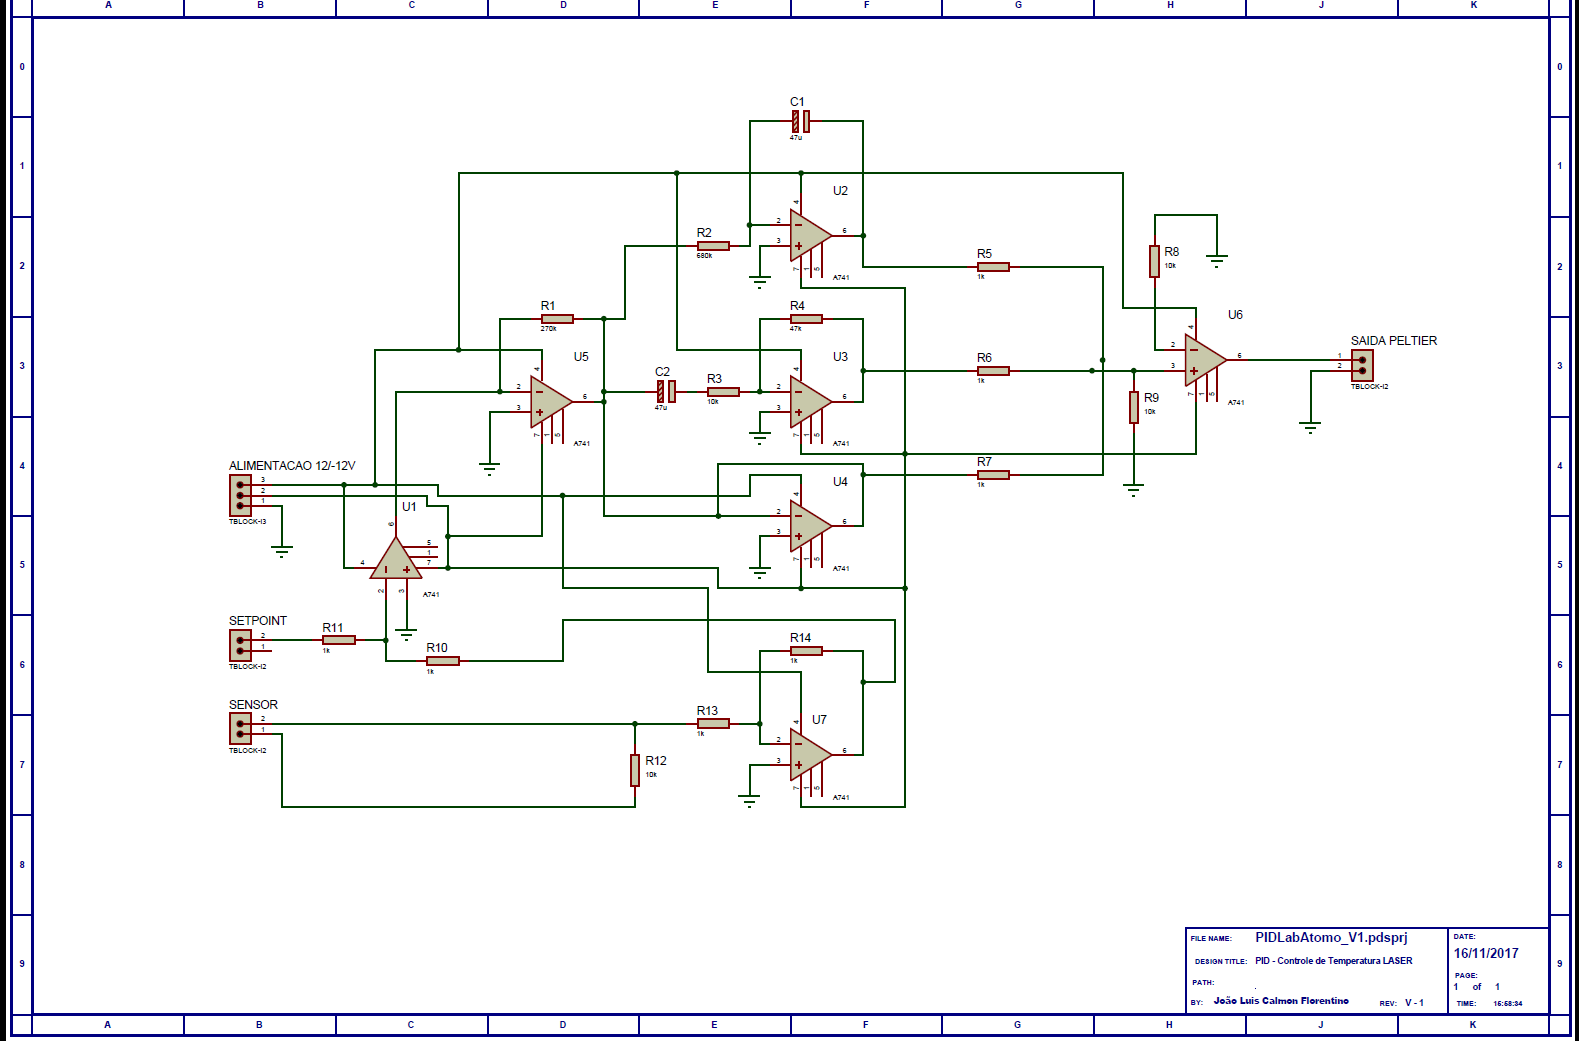
\includegraphics[width=0.8\linewidth]{./ima/esquemaCirucito-02.png}
		%\caption{}
		\label{fig:esquema}
		\caption{Esquema de Circuito}
	\end{figure}

Após a montagem deste esquema no software, fez-se a montagem da placa PCB para este arranjo de circuito. \\
Este programa, após a elaboração do layout do circuito, possibilita uma visualização da placa montada, que resultou no seguinte layout:\\
\begin{figure}[H]
		\centering
		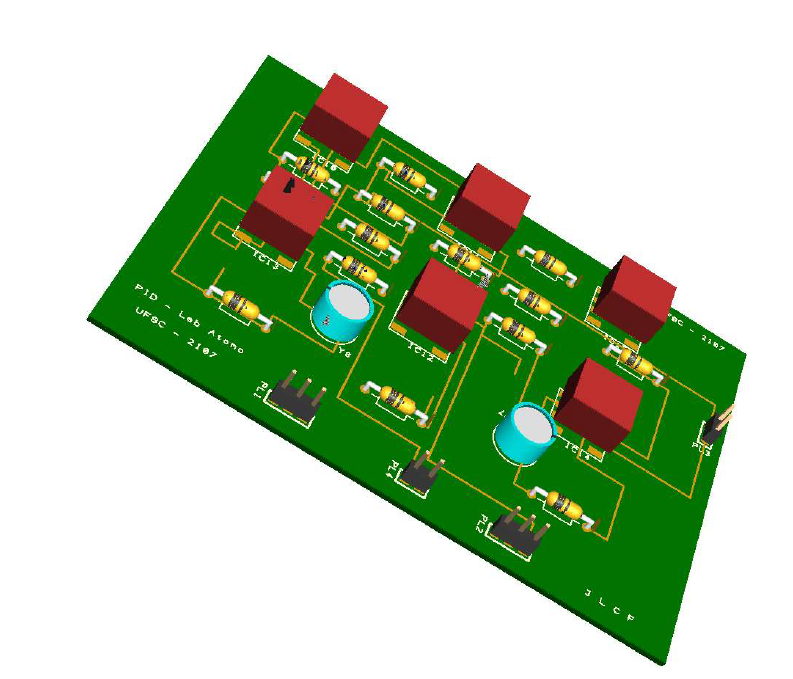
\includegraphics[width=0.7\linewidth]{./ima/Layout-01.png}
		%\caption{}
		\label{fig:Layout da placa de circuito}
		\caption{Layout de Circuito}
	\end{figure}

\paragraph{Atualização de Projeto:}
Durante a montagem do esquema de circuito, encontrei um circuito integrado, o \emph{Power Drive for Peltier - MAX1968-MAX1969} (ver anexos).\\
Este circuito integrado, vem a ser um \emph{Driver} (circuito dedicado) que fornece a um elemento \emph{Peltier} os parâmetros de polarização necessários para que o mesmo atinja a temperatura ajustada em um \emph{setpoint}.\\

Foram comprados quatro unidades destes integrados para que se possa estudar o circuito, e através do circuito sugerido no \emph{datasheet} do dispositivo montar o mesmo para testes.\\

O circuito sugerido pelo \emph{datasheet} funciona da seguinte maneira: \\
\begin{itemize}
\item \textbf{Funcionamento Básico:}\\

O circuito é energizado em 5V, e o modelo que foi adquirido é capaz de fornecer uma corrente de \textbf{$ \pm $3A}. Esta corrente polariza, de acordo a um sinal de \emph{setpoint} o elemento \emph{Peltier} ligado diretamente ao integrado, com uma corrente positiva, ou negativa, o que possibilita a obtenção de temperaturas negativas e positivas no elemento \emph{Peltier}. \\
Diretamente ao circuito integrado \emph{MAX1968}, também é inserido o circuito responsável pelo sensor de temperatura, o qual, para este projeto, esta sendo usado o \emph{AD 590}.\\
O circuito para este projeto está no anexo, e segue, basicamente, o que esta sugerido no circuito do datasheet (anexo) figura 1, no entanto para o circuito de ajuste do setpoint, será usado um dispositivo \emph{PIC 16F877A} ( Microcontrolador PDIP 40 pinos - carateristicas e funcionalidades no datasheet anexo) que reduzirá consideravelmente o numero de componentes no circuito de ajuste de setpoint bem como proporciona saidas analógicas que será usado no comando do circuito \emph{MAX1968}. Alem disso este Microcontrolador tem um custo reduzido e facilidade de encontrar no mercado ( custo aproximado de catorze Reais).
Este Microcontrolador é programado via software linquagem C, gravado no  dispositivo e pode ser alterado a qualquer instante, para aperfeiçoamento ou mesmo correções e manutenções. A rotina de programação também está nos anexos deste trabalho. \\

\begin{figure}[H]
		\centering
		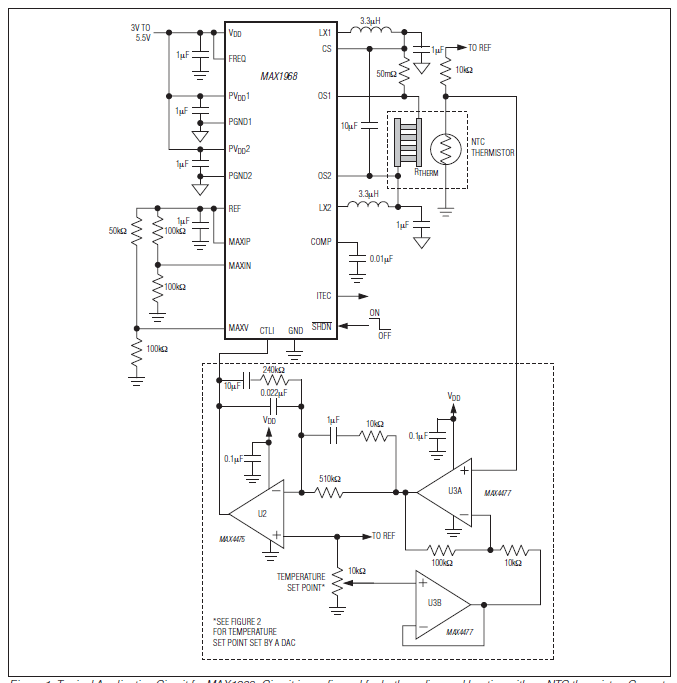
\includegraphics[width=0.7\linewidth]{./ima/esquemaDataSheet01.png}
		%\caption{}
		\label{fig:esq DataSheet}
		\caption{Esquema Datasheet - fig 1}
	\end{figure}

\item \textbf{Componentes e características do circuito:}\\

O Circuito projetado terá 02 botões de ajuste de temperatura, de forma digital, iniciando a marcação em zero grau, e após o ajuste desejado, um botão que iniciará o ciclo. \\
A temperatura ajustada (que será o \emph{setpoint})será visualizado em um painel de display de 7 segmentos, com marcação de temperatura negativa e 02 dígitos decimais e 02 dígitos para os milésimos formando, por exemplo o ajuste de $ -10.05 ºC $ no painel.\\
O dispositivo \emph{MAX1968} possui internamente, em sua implementação, o recurso de\emph{ PID }, recurso esse que vinha a ser o objetivo desse trabalho. Este elemento de circuito mantém  a temperatura do ajustada no \emph{setpoint}, desta forma não é necessário um circuito paralelo de \emph{PID }. Todas essas características e funcionalidades serão testadas no protótipo do circuito. \\


\end{itemize}

Nesta etapa do trabalho, estou usando o \emph{software PROTEUS \copyright  } versão 8 professional  para desenvolvimento do esquema de circuitos, testes eletrônicos via software e implementação da placa de PCI. \\

 